\section{Grundlagen} %%Hier müssten wir eigentlich eine Unterkategorie mit MOOC und ISSuccess einführen...
\label{sec:grundlagen}
Es war das Jahr 2008, als George Siemens und Stephen Downes an der Universität Manitoba in Kanada eine Vorlesung über das Internet verbreiteten und dabei über 2200 Teilnehmer von der ganzen Welt erreichen konnten. Dieses Ereignis ging als der erste Massive Open Online Course in die Geschichte ein. Jeder Interessierte konnte damals ohne jegliche Kosten an dem Kurs teilnehmen. Diese Idee entwickelte sich in den folgenden Jahren weiter und ab 2011 begannen die ersten US-amerikanischen Universitäten den eigenen Studierenden MOOCs als Erweiterungsangebot anzubieten. Seitdem bieten die meisten Universitäten eigene MOOCs an, welche sich dabei meist an externe Personen richten. Darüber hinaus gibt es unterschiedliche Unternehmen, die eigene MOOCs anbieten. In der Regel ist die Teilnahme an einem MOOC kostenlos, die Ausstellung eines Zertifikats inklusive Credit Points nach erfolgreicher Teilnahme jedoch nur gegen Gebühr möglich.
\newline 
Auch die Leuphana Universität Lüneburg bietet mit der Digital School Massive Open Online Courses an. Dabei werden unterschiedliche Kooperationspartner wie unter anderem das Goethe-Institut mit einbezogen.
\newline 
Da historisch gesehen e-Learning Anwendungen vor der Etablierung von MOOCs genutzt wurden, sind in der wissenschaftlichen Literatur dazu Ergebnisse und Best Practice Beispiele für umfangreiche Analysen vorhanden. Häufig wird dabei auf ein Modell von DeLone und McLean zurückgegriffen \parencite[vgl.]{mohammadi2015factors, freeze2010success}, welches international unter dem Namen "`IS Success Model"' bekannt ist. Die Erfolgsmessung von Informationssystemen verfolgt dabei einem bestimmten Muster und ermöglicht somit Vergleiche mit anderen Erhebungen. Seit der ersten Entwicklung im Jahr 1992 wurde das Modell intensiv diskutiert und dabei empirisch auf die Qualität hin überprüft. Grundlegend stellten DeLone und McLean fest, dass sich fast alle Erfolgsmessungen in nur sechs Kategorien einordnen lassen, die untereinander als abhängige Variablen dargestellt werden können. Im Laufe der wissenschaftlichen Weiterentwicklung wird in der Literatur das aktuelle Modell - wie in Abbildung \ref{IS Success Model} grafisch dargestellt - verwendet. \parencite[vgl.]{delone2002information})

\begin{figure}[h]
\centering
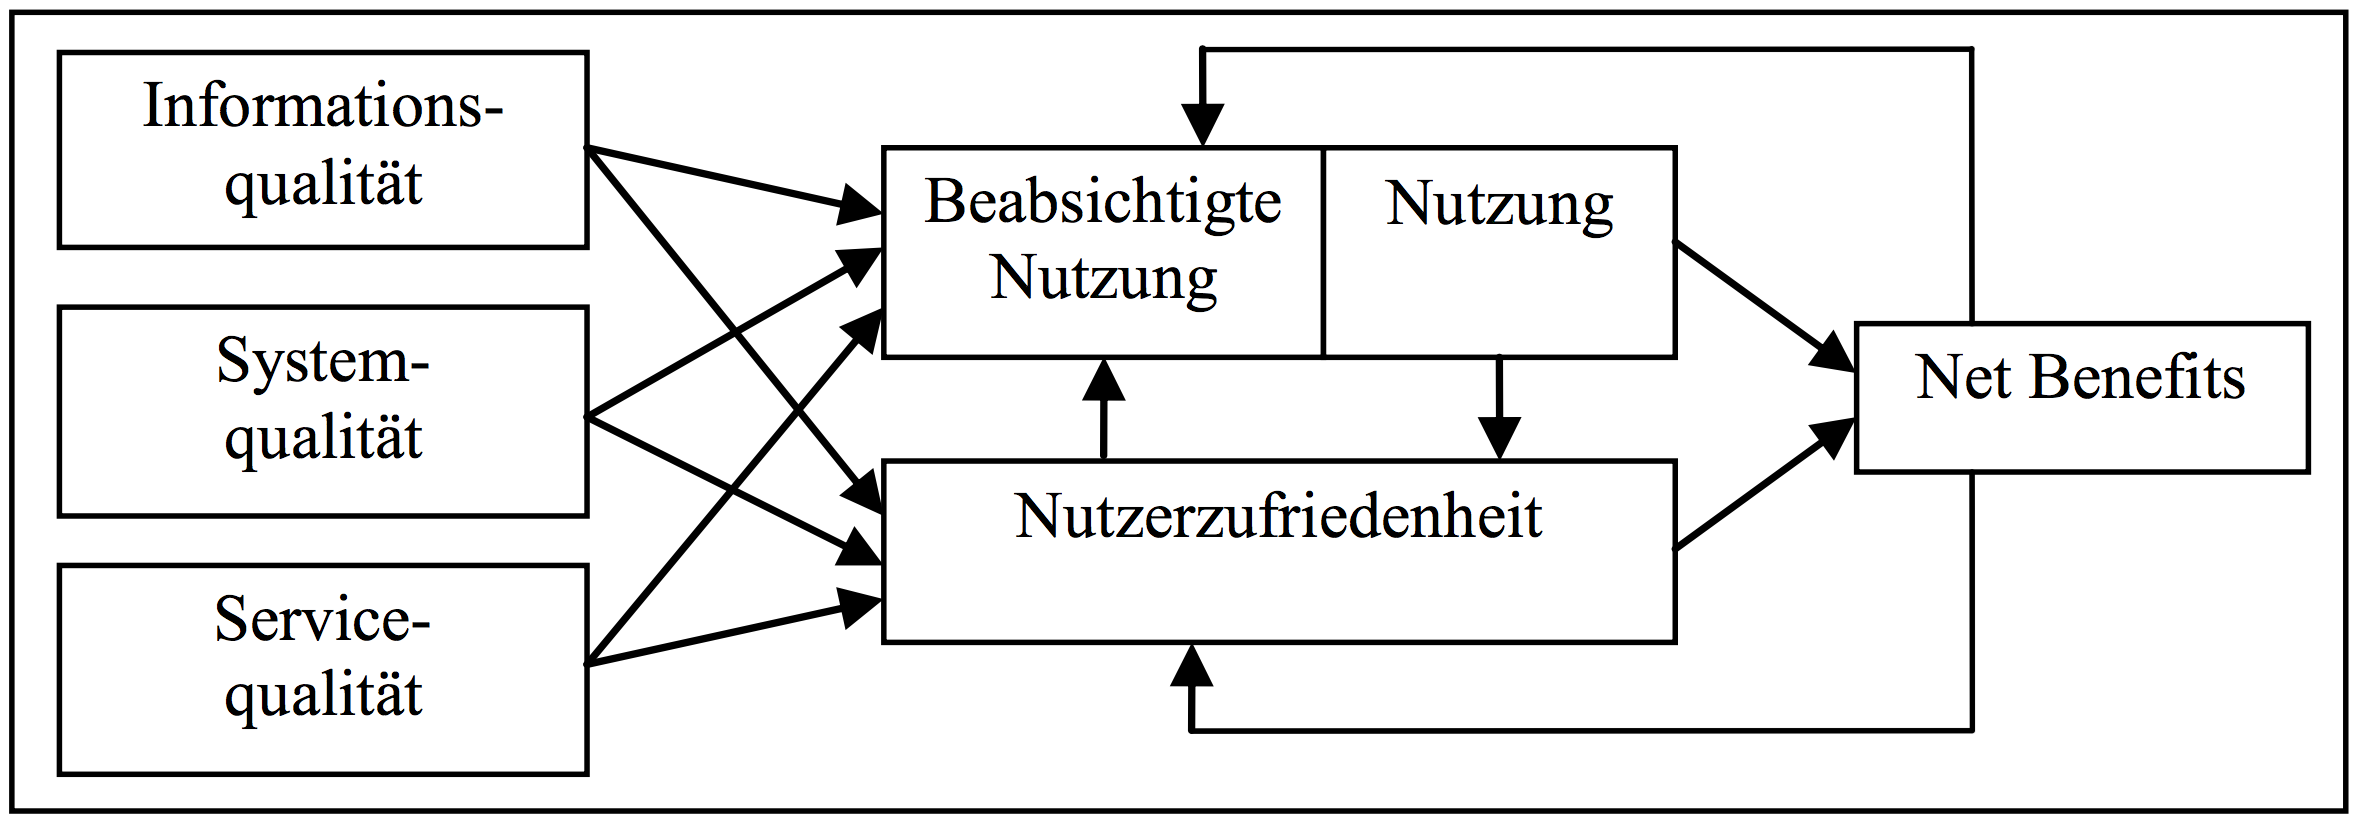
\includegraphics[width=1\textwidth]{Grafiken/issuccess.png}
\caption{IS Success Modell}
\label{IS Success Model}
\end{figure}


%\cite{king2006meta} sagten:" \blindtext" \parencite{behrenbruch2013understanding}